\documentclass[review]{elsarticle}

\usepackage{lineno,hyperref}
\modulolinenumbers[5]

\journal{Journal of \LaTeX\ Templates}

%%%%%%%%%%%%%%%%%%%%%%%
%% Elsevier bibliography styles
%%%%%%%%%%%%%%%%%%%%%%%
%% To change the style, put a % in front of the second line of the current style and
%% remove the % from the second line of the style you would like to use.
%%%%%%%%%%%%%%%%%%%%%%%

%% Numbered
%\bibliographystyle{model1-num-names}

%% Numbered without titles
%\bibliographystyle{model1a-num-names}

%% Harvard
%\bibliographystyle{model2-names.bst}\biboptions{authoryear}

%% Vancouver numbered
%\usepackage{numcompress}\bibliographystyle{model3-num-names}

%% Vancouver name/year
\usepackage{numcompress}\bibliographystyle{model4-names}\biboptions{authoryear}

%% APA style
%\bibliographystyle{model5-names}\biboptions{authoryear}

%% AMA style
%\usepackage{numcompress}\bibliographystyle{model6-num-names}

%% `Elsevier LaTeX' style
\bibliographystyle{elsarticle-num}
%%%%%%%%%%%%%%%%%%%%%%%

\graphicspath{{./figure/}}

\usepackage{amsmath}
\usepackage{amssymb}
\usepackage{xeCJK}
\usepackage{enumerate}
\usepackage{amsthm}
\newtheorem{theorem}{Theorem}
\newtheorem{corollary}[theorem]{Corollary}
\newtheorem{lemma}{Lemma}
\newtheorem{example}{Example}
\newtheorem{proofOfTheorem}{Proof of Theorem}
\begin{document}

\begin{frontmatter}

\title{积分似然比检验\tnoteref{mytitlenote}}
\tnotetext[mytitlenote]{Fully documented templates are available in the elsarticle package on \href{http://www.ctan.org/tex-archive/macros/latex/contrib/elsarticle}{CTAN}.}

%% Group authors per affiliation:
\author{author \fnref{myfootnote}}
\address{Radarweg 29, Amsterdam}
\fntext[myfootnote]{Since 1880.}

%% or include affiliations in footnotes:
\author[mymainaddress,mysecondaryaddress]{Elsevier Inc}
\ead[url]{www.elsevier.com}

\author[mysecondaryaddress]{Global Customer Service\corref{mycorrespondingauthor}}
\cortext[mycorrespondingauthor]{Corresponding author}
\ead{support@elsevier.com}

\address[mymainaddress]{1600 John F Kennedy Boulevard, Philadelphia}
\address[mysecondaryaddress]{360 Park Avenue South, New York}

\begin{abstract}
    本文针对一般的检验问题,提出了积分似然比检验方法,得到了其在原假设下的分布和局部功效函数,并在较弱的条件下给出了严格证明。我们的定理可以适用于似然函数有界的情形,由于此时似然比检验不存在,所以理论上积分似然比检验可以解决一些似然比检验无法解决的问题。而实际上,混合正态模型正好是这样的例子,积分似然比检验水平控制的很好,而对应的,似然比统计量甚至不存在。在我们的定理无法应用的情形,比如高维情形,积分似然比方法仍然是一种寻找检验的优良方法。我们考虑了高维均值检验问题,此时似然比检验不存在,而积分似然比方法依然存在,所以可以作为似然比检验在高维情形下的一种替代品,它具有类似似然比检验的优良性质,模拟结果显示在一些情形下,它优于已有的检验方法。
\end{abstract}

\begin{keyword}
\texttt{elsarticle.cls}\sep \LaTeX\sep Elsevier \sep template
\MSC[2010] 00-01\sep  99-00
\end{keyword}

\end{frontmatter}

\linenumbers

\section{介绍}

 \cite{Aitkin1991Posterior}针对检验问题$H_0:\theta\in \Theta_0$ vs $H_1:\theta\in \Theta_1$提出了后验贝叶斯因子,形式是
\begin{equation}
    \frac{\int_{\Theta} p(X|\theta)\pi(\theta|X)\, d\theta}{\int_{\Theta_0}p(X|\theta)\pi^*(\theta|X)\, d\theta}
\end{equation}
其中$X=X_1,\cdots,X_n$是观测数据, $p(x|\theta)$是样本密度, $\pi^*(\theta|x)$是原假设下的后验密度,$\pi(\theta|x)$是被择假设下的后验密度。
\cite{gelfand1993bayesian}利用了拉普拉斯近似求得了它在原假设的分布。他们的方法并没有显式的给出定理成立需要的条件,而且证明依赖于拉普拉斯近似,这就假设了极大似然估计的存在。而当极大似然估计存在时,似然比检验也存在。所以他们的结论并没有显示出后验贝叶斯因子比似然比检验更为广泛的适用性。

基于后验贝叶斯因子,我们考虑更一般的积分似然比检验统计量:
\begin{equation}
    \Lambda (X)=\frac{\int_{\Theta} p(X|\theta)\pi(\theta;X)\,d\theta}{\int_{\Theta_0} p(X|\theta)\pi^*(\theta;X)\,d\theta}
\end{equation}
其中$\pi(\theta;X)$和$\pi^*(\theta;X)$是基于数据的权函数,但不必等于后验密度。

似然比检验是被最广泛使用的统计方法,它具有很多最优性质,比如由NP引理,它在简单原假设和简单被择假设下是最有效检验,见\cite{Lehmann}。在多维情形,一般是没有最有效检验的,但是似然比检验是在Bahadur efficiency的意义下是渐进最优的,见\cite{MR0315820}。而我们知道在许多模型中,即使是一些被广泛使用的模型,似然也经常是是无界的,见\cite{Cam1990Maximum}。这种情形下,似然比检验不存在。但此时积分似然比检验是可能存在的,比如后面我们举的例子。

参考Bernstein-von Mises定理的证明,见\cite{van2000asymptotic},本文在很一般的假设下证明积分似然比检验的Wilks现象及局部功效,尤其是我们的定理不要求似然函数有界,这使得我们的方法可以用于一些似然无界在的模型。并举例说明其广泛的适用性。

\section{积分似然比检验}

设$X_1,\cdots,X_n$ i.i.d. 服从$P_{\theta}:\theta\in\Theta$,设$X=(X_1,\cdots,X_n)$为随机样本,设全空间$\Theta$是$\mathbb{R}^{p_2}$的一个开子集,我们设原空间$\Theta_0$是$\Theta$的一个$p_1$维子空间,准确来说,我们定义
\begin{equation}
    \Theta_0=\{\theta\in\Theta:\theta_{p_1+1}=\theta_{0,{p_1+1}},\cdots,\theta_{p_2}=\theta_{0,{p_2}}\} 
\end{equation}
也就是说后$p_2-p_1$维$(\theta_{0,{p_1+1}},\cdots,\theta_{0,{p_2}})$固定,是我们想要检验的参数,前$p_1$维是讨厌参数。我们的问题是检验
\begin{equation}
H_0:\theta\in \Theta_0\quad vs. \quad H_1:\theta\in \Theta
\end{equation}

由于在$\Theta_0$中的$\theta$只有前$p_1$个参数变化,$\Theta_0$可以看成是$\mathbb{R}^{p_1}$空间的一个开子集,为了记号方便,我们定义$\Theta^*_0=\{(\theta_1,\cdots,\theta_{p_1})^T:\, (\theta_1,\cdots,\theta_{p_1},\theta_{0,p_1+1},\theta_{0,p_2})\in \Theta_0\}$,故我们可以用$p_1$维向量 $\theta^*\in
\Theta_0^*$表示$\theta\in\Theta_0$并把$\Theta_0^*$看成原空间。我们下面会根据上下文使用原空间的记号。我们在全空间$\Theta$和原空间$\Theta_0^*$里分别设置可以依赖于数据的权函数$\pi(\theta;X)$和$\pi^*(\theta^*;X)$,则积分似然比统计量定义为:
\begin{equation}\label{likelihoodRatio}
    \Lambda (X)=\frac{\int_{\Theta} p(X|\theta)\pi(\theta;X)\,d\theta}{\int_{\Theta^*_0} p(X|\theta^*)\pi^*(\theta^*;X)\,d\theta^*}
\end{equation}

说一说在极限试验的意义下的解释。

\section{主要结果}

下面记$\rightsquigarrow$代表弱收敛,
$dN(\mu,\Sigma)(h)$是一个均值为$\mu$,方差为$\Sigma$的正态密度在$h$处的取值。

设$\theta_0\in\Theta_0$是原假设中一个固定的参数,我们研究积分似然比统计量在$\theta_0$处(及其附近)的渐进性质。
设试验$P_\theta : \theta\in \Theta$在$\theta_0$处均方可微,即存在随机$\dot{\ell}_{\theta_0}$使得
\begin{equation}
    \int \big[\sqrt{p_{\theta_0+h}}-\sqrt{p_{\theta_0}}-\frac{1}{2}h^T\dot{\ell}_{\theta_0}\sqrt{p_{\theta_0}}\big]^2\, d\mu=o(\|h\|^2),\quad h\to 0
\end{equation}
其中$\mu$是$P_{\theta}$的控制测度。而$p_{\theta}(x)$是$P_{\theta}(x)$相对于$\mu$的密度函数。$\dot{\ell}_{\theta_0}$是均方可微意义下的得分函数。

设$I_{\theta_0}=P_{\theta_0}\dot{\ell}_{\theta_0}\dot{\ell}_{\theta_0}^T$是$\theta_0$处均方可微意义下的信息阵,
设“局部充分统计量”$\Delta_{n,\theta_0}=\frac{1}{\sqrt{n}}\sum_{i=1}^n I_{\theta_0}^{-1}\dot{\ell}_{\theta_0}(X_i)$。相对应的,在原空间中$\dot{\ell}^*$,$I^*_{\theta_0}$,$\Delta_{n,\theta_0}^*$均可同样定义。我们很容易知道,$\dot{\ell}^*_{\theta_0}$是$\dot{\ell}_{\theta_0}$的前$p_1$维向量,$I^*_{\theta_0}$是$I_{\theta_0}$左上角的$p_1\times p_1$维矩阵,$\Delta_{n,\theta_0}^*=\frac{1}{\sqrt{n}}\sum_{i=1}^n I_{\theta_0}^{*-1}\dot{\ell}^*_{\theta_0}(X_i)$

设$h=\sqrt{n}(\theta-\theta_0)$,$h$把参数$\theta$在$\theta_0$附近以$\sqrt{n}$的比例重参数化。易知在原假设下$h=0$,而研究局部被择下,一般会让$h$趋于某个常数。

下面是我们定理需要的正规条件:

\begin{enumerate}[(i)]
    \item
        设Bernstein-von Mises定理(见\cite{van2000asymptotic})的条件满足: $\Theta$是$\mathbb{R}^p$的开子集,试验($P_{\theta}:\theta\in\Theta$)在$\theta_0\in \Theta$处均方可微,具有非奇异信息阵$I_{\theta_0}$,假设对任意的$\epsilon>0$,存在一个相合检验序列:
        \begin{equation}
            P_{\theta_0}^n\phi_n\to 0,\quad \sup_{\|\theta-\theta_0\|\geq \epsilon} P_\theta^n(1-\phi_n)\to 0.
        \end{equation}
        设$\pi_n(h;X)$是一个满足Bernstain-von Mises定理结论的权函数:
        \begin{equation}
            \|\pi_n(h;X)-dN(\Delta_{n,\theta_0},I_{\theta_0}^{-1})(h)\|\overset{P_{\theta_0}^n}{\to}0
        \end{equation}
    \item
        $\pi_n(h;X)$的支撑在$\|h\|\leq K\sqrt{n}$上,$K$是一个固定常数。$\sup_h |\pi_n(h;X)|\leq A$对某个$A$依概率成立。
    \item
        存在$\theta_0$的某个邻域$V$和某个函数$\dot{\ell}$满足$P_{\theta_0}\dot{\ell}^2<\infty$,对$\forall \theta_1,\theta_2\in V$,有
        \begin{equation}
            |\log p_{\theta_1}(x)-\log p_{\theta_2}(x)|\leq \dot{\ell}(x)\|\theta_1-\theta_2\|.
        \end{equation}
\end{enumerate}

条件$(i)$是很弱的条件。条件(ii)中的支撑条件可以等价的表述为$\pi_n(h;X)$作为$\theta$的函数,其支撑有界。对于一个统计模型,我们通常认为似然函数在很远处的取值没有太大意义,所以不分配权是合理的。因为我们不该某个$\theta$附近分配过大的权,所以权函数有界的条件也是合理的。事实上,我们总可以把后验密度$\pi_n(h|X)$改造成满足条件$(ii)$的权函数$\pi_n(h;X)$,比如我们选取一个充分大的$M$,则容易证明
\begin{equation}
    \pi_n(h;X)=\min(\pi_n(h|X),M) 1_{\|h\|\leq K\sqrt{n}}
\end{equation}
同时满足条件$(i)$,$(ii)$。而且我们有理由相信这样得到的权函数比后验密度收敛的更快一点。
均方可微条件使得似然可以在$\theta_0$的邻域内展开,我们在证明一般性的定理时需要把似然函数在$\theta_0$的邻域内一致展开,所以我们需要条件$(iii)$。

我们的第一个定理是
\begin{theorem}\label{theoremMain}
    如果条件$(i)$,$(ii)$,$(iii)$满足,设$\eta_n$是有界实数序列,那么我们有
%    \begin{equation}
%        \Big|\int_{\mathbb{R}^{p}}\frac{p_h(X)}{p_0(X)}\pi_n(h;X)\,dh-\int_{\mathbb{R}^{p}}e^{h^TI_{\theta_0}\Delta_{n,\theta_0}-\frac{1}{2}h^TI_{\theta_0}h}dN(\Delta_{n,\theta_0},I_{\theta_0}^{-1})(h)\,dh\Big|\xrightarrow{P_{\eta_n}^n}0
%    \end{equation}
    \begin{equation}
        \Big|\int_{\mathbb{R}^{p}}\frac{p_h(X)}{p_0(X)}\pi_n(h;X)\,dh-
        2^{-\frac{p}{2}}e^{\frac{1}{2}\Delta_{n,\theta_0}^TI_{\theta_0}\Delta_{n,\theta_0}}
        \Big|\xrightarrow{P_{\eta_n}^n}0
    \end{equation}
\end{theorem}
基于定理\ref{theoremMain},我们可以得到积分似然比统计量在原假设的渐进分布,也就是wilks现象。我们可以根据此渐进分布来决定检验的临界值
\begin{theorem}\label{theoremWilks}
    设定理\ref{theoremMain}的条件对原空间$\Theta_0$和全空间$\Theta$均成立,真实参数$\theta_0$是$\Theta$的一个内点,同时是$\Theta_0$的一个相对内点,那么我们有
\begin{equation}
    2\log(\Lambda(X))\overset{P_0^n}{\rightsquigarrow} \chi^2_{p_2-p_1}-(p_2-p_1)\log(2)
\end{equation}

\end{theorem}


有了定理\ref{theoremMain},我们可以利用Le Cam第三引理得到积分似然比统计量在局部被择下的渐近分布:
\begin{theorem}   \label{theoremPower}
    设定理\ref{theoremMain}的条件对原空间$\Theta_0$和全空间$\Theta$均成立。$\theta_0$是$\Theta_0$的一个内点,同时是$\Theta_0$的一个相对内点。真实参数$\theta$满足$\eta_n=\sqrt{n}(\theta-\theta_0)\to \eta$。若
\begin{equation}
    I_{\theta_0}=\left(
        \begin{matrix}
            I^*_{\theta_0}&I_{12}
            \\
            I_{21}&I_{22}
        \end{matrix}
    \right)
\end{equation}
$I_{22\cdot 1}=I_{22}-I_{21}I_{\theta_0}^{*-1}I_{12}$
    那么我们有
\begin{equation}
    2\log(\Lambda(X))\overset{P_0^n}{\rightsquigarrow} \chi^2_{p_2-p_1}(\delta)-(p_2-p_1)\log(2)
\end{equation}
其中
\begin{equation}
\delta=\eta^T
    \left(
        \begin{matrix}
            0&0\\
            0&I_{22\cdot 1}
        \end{matrix}
    \right)
    \eta
\end{equation}
\end{theorem}

我们的结果和似然比检验结果很类似。这样的结果可以从试验的收敛的观点来解释。从渐进的角度来讲,我们在$n$个样本空间中的统计问题近似于只观测到一个量$\Delta_{n,\theta_0}$。而在$h_n\to h$时,$\Delta_{n,\theta_0}\rightsquigarrow N(h,I_{\theta_0}^{-1})$。所以问题可以近似为只有一个观测$X\sim
N(h,I_{\theta_0}^{-1})$的问题。在这种情形下,我们可以直接计算似然比统计量,正是我们定理的结论。这样我们定理的结论就没什么奇怪的了。

\section{混合正态分布}
\cite{Cam1990Maximum}给出了一些似然无界的例子。混合正态分布是其中给出的第一个例子。这一节通过这个例子来说明积分似然比方法的优越性。

设$X_1,\cdots,X_n$ i.i.d. 服从混合正态分布
\begin{equation}
    \frac{1-\alpha}{\sqrt{2\pi}}\exp\left\{-\frac{1}{2}(x-\mu)^2\right\}+
    \frac{\alpha}{\sigma\sqrt{2\pi}}\exp\left\{-\frac{1}{2}\frac{(x-\mu)^2}{\sigma^2}\right\}
\end{equation}
其中$\alpha$是已知的固定参数。参数空间设为
\begin{equation}
    \Theta=\{\theta=(\mu,\sigma^2)^T:\mu\in(\-\infty,\infty),\sigma^2\in (0,M)\}
\end{equation}
\cite{Cam1990Maximum}指出,在这个模型下,似然函数是无界的。事实上,令$\mu=X_1$,然后令$\sigma^2\to 0$,则似然函数趋于无穷。

现在我们在这个模型下考虑检验问题$H_0:\mu=0,\sigma=2$ vs $H_1:\theta\in
\Theta$。似然比检验显然已经失效了,但此时积分似然比统计量仍然可以使用。事实上,我们可以验证(虽然很繁琐)条件$(i)$,$(ii)$,$(iii)$均成立,所以定理\ref{theoremWilks}和\ref{theoremPower}均成立。当然要想使用积分似然比统计量,我们需要寻找权函数,在这个例子中我们考虑用后验密度。这里我们可以看出,假设我们先验设置成无信息先验,那么后验密度与似然函数成正比,所以是无界的。无界的权函数不仅会使得我们的定理条件$(ii)$无法满足,更重要的是,在积分似然比统计量中,它会给似然函数在没意义的地方设置过多的权重,而我们实际上期望权函数集中在真实参数附近,所以无界的权函数使得统计量的性质变得很复杂并且收敛速度变慢。一种解决这个问题的方法是按照前面提到的,选取一个合适的充分大的$M^*$,定义新的权函数为
\begin{equation}
    \min(\pi_n(h;X),M^*)
\end{equation}
则新的有界的权函数依然满足条件$(i)$,甚至表现的更好。而条件$(ii)$也满足了。

在我们这个例子中,我们并不需要这样解决权函数无界的问题。因为我们只要设置合适的先验分布,后验密度就会有界,这样我们仍然可以使用后验密度作为权函数。我们发现当$\mu=X_1$, $\sigma^2\to 0$时,似然趋于无穷的速度正比例于$\frac{1}{\sigma}$。所以我们设置合适的先验对冲掉这个量。容易看出,$\chi^2(3)$的密度函数正好可以做到这一点。

故我们设先验是
\begin{equation}
    dN(0,1)(\mu)\times d\chi^2(3)(\sigma^2)
\end{equation}
其中$d\chi^2(3)(\sigma^2)$代表自由度为$3$的$\chi^2$分布的密度函数在$\sigma^2$处的取值。由于参数空间的限制,$\sigma^2$只在$(0,M)$上取值,所以这个先验并不是个概率密度,但这并不妨碍我们求得后验密度并计算积分似然比统计量。

我们下面通过数值模拟验证Wilks现象。我们取样本量$n=50,100,200$和超参数$\alpha=0.1,0.5,0.9$。每种情况重复抽取$1000$次样本,得到$1000$个积分似然比统计量。理想情况应该是它们的样本与$\chi^2(2)$的分布很接近。我们画出样本分布相对于$\chi^2(2)$分布的QQ图,模拟显示样本分布与$\chi^2(2)$分布很接近,见下图:

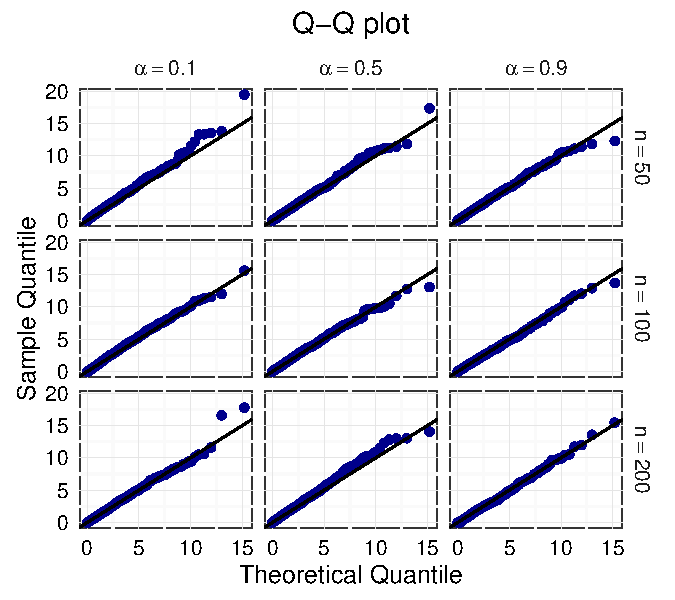
\includegraphics{myQQPlot.pdf}



\section{高维正态均值检验}
在一些问题中,我们可以直接使用积分似然比方法:直接验证条件$(i)$,$(ii)$,$(iii)$,然后直接利用wilks现象来求得积分似然比检验的临界值。但是我们在一般性定理在一些情形下不能适用,比如高维问题($p\to \infty$)。但此时积分似然比仍是一种寻找检验统计量的方法,并且我们发现用积分似然比方法得到的统计量仍然具有很多优点。

设$X_1,\cdots,X_n\in \mathbb{R}^p$ i.i.d. 服从$N(\mu,\Sigma)$,方差未知,$p$随$n\to \infty$而趋于无穷。我们考虑均值检验问题$H_0:\mu=0$ vs $H_1:\mu\in \mathbb{R}^p$

这个问题的似然比统计量是著名的Hotelling $T^2$统计量。但是当$p>n$时,由于样本协方差矩阵不可逆,Hotelling $T^2$统计量不存在。高维情形下的均值检验问题被很多学者研究过了,比如\cite{Bai1996Effect},他们的提出统计量
\begin{equation}
    T_{B}=\frac{n\|\bar{X} \|^2-tr S}{
        \sqrt{\frac{2(n-1)n}{(n-2)(n+1)}(tr S^2-\frac{(tr S)^2}{n-1})}
    }
\end{equation}
其中$S=\frac{1}{n}(X_i-\bar{X})(X_i-\bar{X})^T$是样本协方差矩阵。他们在一些假设下证明了$T_B$在原假设下渐近服从$N(0,1)$分布。
我们知道在这个问题上,由于它是多维的检验问题,所以不存在一个检验一致的优于别的检验。
和经典Hotelling方法最显著的不同是他们去掉了协方差的信息,这使得他们的统计量不能根据数据自适应的分配功效的方向,而是把所有的方向相同的对待,而这对于数据的尺度不一,或者分量间有相关性的情形会产生严重的功效损失。一般来说,似然比统计量可以克服上述问题。但是当$p>n$时,似然比检验不存在,这是很可惜的。我们发现虽然似然比检验不存在,但是积分似然比检验存在。我们取后验密度为积分似然比的权函数。

设$W^{-1}(\Psi,m)$是参数为$\Psi$,自由度为$m$的逆威沙特分布,$w^{-1}(B|\Psi,m)$是对应的密度在$B$处的取值。

在$H_0$下,我们设置先验为$\Sigma\sim W^{-1}(\Sigma|I_{p\times p},m)$,其中$I_{p\times p}$是$p$维单位矩阵。计算之后,我们得到\eqref{likelihoodRatio}式分母为一个常数(不依赖于参数与数据)乘以
\begin{equation}\label{highDe}
    \frac{
        |I_{p\times p}+\sum^n_{i=1} X_i X_i^T|^{\frac{1}{2}(n+m)}
    }{
        |I_{p\times p}+2\sum^n_{i=1} X_i X_i^T|^{\frac{1}{2}(2n+m)}
    }
\end{equation}

在$H_1$下,我们对$\Sigma$设置相同的先验,对$\mu$设置条件正态分布:
\begin{equation}
    \pi(\mu,\Sigma)=dN(0,\Sigma/K)(\mu)\times w^{-1}(\Sigma|I_{p\times p},m)
\end{equation}
其中$K$是一常数,则计算得到\eqref{likelihoodRatio}式的分子为一个常数乘以
\begin{equation}\label{highNu}
    \frac{
        |I_{p\times p}+\sum^n_{i=1} (X_i-\bar{X}) (X_i-\bar{X})^T+\frac{nK}{n+K}\bar{X}\bar{X}^T|^{\frac{1}{2}(n+m)}
    }{
        |I_{p\times p}+2\sum^n_{i=1} (X_i-\bar{X}) (X_i-\bar{X})^T+\frac{2nK}{2n+K}\bar{X}\bar{X}^T|^{\frac{1}{2}(2n+m)}
    }
\end{equation}
则我们得到积分似然比统计量为$\frac{\eqref{highNu}}{\eqref{highDe}}$,如果去掉统计中所有的$I_{p\times p}$,则它与Hotelling统计量等价。我们发现积分似然比统计量即使当$p>n$时也存在。为了清楚,设$K=0$,并对统计量进行近似:
\begin{equation}
    \begin{aligned}
        \eqref{highDe}&\approx   2^{-\frac{1}{2}(2n+m)}|I_{p\times p}+\sum^n_{i=1} X_i X_i^T|^{-\frac{n}{2}}
    \\
    \eqref{highNu}&\approx   2^{-\frac{1}{2}(2n+m)}|I_{p\times p}+\sum^n_{i=1} (X_i-\bar{X}) (X_i-\bar{X})^T|^{-\frac{n}{2}}
    \end{aligned}
\end{equation}
如果这样近似,积分似然比统计量等价于
\begin{equation}\label{equation:simpleHighDimension}
    \bar{X}^T(\frac{1}{n}I_{p\times p}+S)^{-1}\bar{X}
\end{equation}
其中$S=\frac{1}{n}(X_i-\bar{X})(X_i-\bar{X})^T$是样本协方差矩阵。

由于在高维情形下我们的定理\ref{theoremWilks}失效。所以我们用\cite{Zhao2016A}中提出的randomization procedure决定检验的临界值。

\cite{Bai1996Effect}的统计量中没有对协方差矩阵进行估计,只估计很少的参数使得他们的统计量方差很小,从而功效较好。但是这样做也优缺点:首先,们在Hotelling检验中用单位阵代替了协方差阵的逆的估计,所以他们必须假定真实的协方差阵与单位阵差别不大,否则他们的定理失效。其次,似然比统计量把功效分配在了比较合理的方向,不估计协方差阵就只能自己事先分配一个功效的方向(他们的统计量里,这个方向是$I$),而这在很多情况下会丧失大量信息,因而是不合理的。

我们考虑如下的情形: $\mu=c(1,0.01,\cdots,0.01)^T$, $c$是一个实数。$\Sigma$是对角阵,$diag(\Sigma)=(0.01,1,1,\cdots,1)$。由于第一个分量方差很小,我们显然应该更在意第一个分量方向,只要第一个分量方向的均值稍微远离$0$一点,我们就应该拒绝,所以理想的功效函数对$c$应该很敏感。下面是在功效函数的模拟结果,$n=40$,
$p=100$,对于白的检验,我们使用渐近正态性确定临界值,对于积分似然比统计量\eqref{equation:simpleHighDimension},我们用\cite{Zhao2016A}的方法重复抽样了$B=100$次得到检验$P$-值。我们模拟了$1000$次样本来计算模拟功效函数。我们的模拟结果显示积分似然比检验在这个功效方向上表现很好,而白、陈的统计量则表现没那么好。

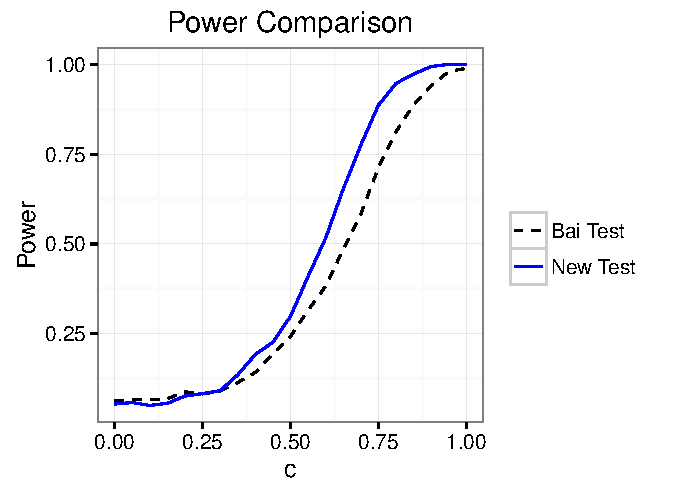
\includegraphics{myPowerFigure.pdf}



\section{Appendix}
对于两个测度序列$P_n$和$Q_n$, $P_n\triangleleft \triangleright Q_n$代表$P_n$和$Q_n$是mutrally contiguous的,即对任意的随即变量序列$T_n$,有$T_n\overset{P_n}{\rightsquigarrow}0\Leftrightarrow T_n\overset{Q_n}{\rightsquigarrow}0$
\begin{lemma}\label{lemmaEx}
    假设$\Theta$是一个$\mathbb{R}^p$的一个开子集并且试验($P_\theta: \theta \in\Theta$)在$\theta_0$处均方可微。那么$P_{\theta_0}\dot{\ell}_{\theta_0}=0$,并且Fisher信息阵$I_{\theta_0}=P_{\theta_0}\dot{\ell}_{\theta_0}\dot{\ell}_{\theta_0}^T$存在。进一步,对于每个收敛序列$h_n\to h$,随着$n\to \infty$,有
    \begin{equation}
        \log \frac{p^n_{h_n}(X)}{p^n_0(X)}=\frac{1}{\sqrt{n}}\sum^n_{i=1}h^T\dot{\ell}_{\theta_0}(X_i)-\frac{1}{2}h^TI_{\theta_0}h+o_{P_{\theta_0}}(1)
    \end{equation}
    见\cite{van2000asymptotic}
\end{lemma}



\begin{lemma}\label{lemmaContiguity}
    设引理\ref{lemmaEx}条件满足。假设$T_n$是一个统计量序列,$U$是一个以原点为中心的球。则
    对任意的随机变量序列$T_n$, $T_n\overset{P^n_0}{\rightsquigarrow}0\Leftrightarrow T_n\overset{P^n_U}{\rightsquigarrow}0$,其中
\begin{equation}
    p^n_U(x)=\frac{1}{V(U)}\int_{U}p_h^n(x)dh
\end{equation}
$V(U)$是球$U$的体积。
\end{lemma}

\begin{proof}
    事实上,我们只需证明
\begin{equation}
\int_{A_n}p_0^n(x)\, d\mu \to 0 \Leftrightarrow \int_{A_n}\frac{1}{V(U)}\int_U p_h^n(x) dh \, d\mu \to 0
\end{equation}
或者
\begin{equation}\label{eq:1}
\int_{A_n}p_0^n(x)\, d\mu \to 0 \Leftrightarrow \int_{U}\int_{A_n} p_h^n(x) d\mu \, dh \to 0
\end{equation}
在引理\ref{lemmaEx}的条件下,对于每个有界序列$h_n$,我们有$P_{h_n}^n\triangleleft \triangleright P_{0}^n$, 也就是
\begin{equation}\label{eq:2}
\int_{A_n}p_0^n(x)\, d\mu \to 0 \Leftrightarrow \int_{A_n} p_{h_n}^n(x) d\mu  \to 0
\end{equation}
我们又知道,存在$\overline{h}_n$ 使得
\begin{equation}
\int_{U}\int_{A_n} p_h^n(x) d\mu \, dh
\leq V(U)\sup_{h}\int_{A_n} p_h^n(x) d\mu
\leq V(U)(\int_{A_n}p^n_{\overline{h}_n}(x)d\mu +1/n)
\end{equation}
类似的我们也有下界。综上
\begin{equation}\label{eq:3}
 V(U)(\int_{A_n}p^n_{\underline{h}_n}(x)d\mu +1/n)
\leq \int_{U}\int_{A_n} p_h^n(x) d\mu \, dh
\leq V(U)(\int_{A_n}p^n_{\overline{h}_n}(x)d\mu +1/n)
\end{equation}
由\eqref{eq:2} 和\eqref{eq:3}, \eqref{eq:1} 成立
\end{proof}

\begin{lemma}\label{lemmaTest}
设试验($P_\theta :\theta\in \Theta$) 在$\theta_0$处均方可微,具有非奇异的Fisher信息阵$I_{\theta_0}$, 假设对每个$\epsilon>0$, 存在一个检验序列$\phi_n$ 使得
$$
P_{\theta_0}^n \phi_n \to 0,\quad \sup_{\|\theta-\theta_0\|\geq \epsilon}P_{\theta}^n (1-\phi_n)\to 0
$$
那么,设$M_n\to \infty$,则存在一个检验序列 $\phi_n$ 和一个常数$c>0$ 使得对每个充分大的$n$ 和每个$\theta$使得$\|\theta-\theta_0\|\geq M_n /\sqrt{n}$,我们有
$$
P_{\theta_0}^n\phi_n \to 0, \quad P_\theta^n (1-\phi_n)\leq e^{-cn(\|\theta-\theta_0\|^2\wedge 1)}
$$
见\cite{van2000asymptotic}
\end{lemma}
\begin{lemma}\label{lemmaUniform}
设试验($P_\theta :\theta\in \Theta$) 在$\theta_0$处均方可微,具有非奇异的Fisher信息阵$I_{\theta_0}$, 进一步,假设存在$\theta_0$的某个邻域$V$和某个函数$\dot{\ell}$满足$P_{\theta_0}\dot{\ell}^2<\infty$,对$\forall \theta_1,\theta_2\in V$,有
    \begin{equation}
        |\log p_{\theta_1}(x)-\log p_{\theta_2}(x)|\leq \dot{\ell}(x)\|\theta_1-\theta_2\|.
    \end{equation}
则对每个$M$,有
    \begin{equation}
        \sup_{\|h\|\leq M}\Big|
         \log \frac{p^n_{h_n}(X)}{p^n_0(X)}-\frac{1}{\sqrt{n}}\sum^n_{i=1}h^T\dot{\ell}_{\theta_0}(X_i)+\frac{1}{2}h^TI_{\theta_0}h
        \Big|\xrightarrow{P^n_0}0.
    \end{equation}
\end{lemma}

\begin{proofOfTheorem}
    由Contiguity,我们只需证明命题在$P_0^n$下趋于0。

    证明分两步。第一步,设$C$是一个以$0$为圆心,半径固定为$M$的球,我们证明
\begin{equation}\label{eq:14}
    \left|\int_C \frac{p^n_h(X)}{p^n_0(X)}\pi_n (h;X) \, dh-\int_C e^{h^TI_{\theta_0}\Delta_{n,\theta_0}-\frac{1}{2}h^TI_{\theta_0}h}dN(\Delta_{n,\theta_0},I_{\theta_0}^{-1})(h)\, dh\right|
 \xrightarrow{P^n_0}0
\end{equation}
有引理\ref{lemmaUniform},对每个固定的$M$
\begin{equation}
    \sup_{\|h\|\leq M}|\log \frac{p_h^n(X)}{p_0^n(X)}-h^TI_{\theta_0}\Delta_{n,\theta_0}+\frac{1}{2}h^TI_{\theta_0}h|\xrightarrow{P_0^n}0 
\end{equation}
所以我们有
\begin{equation}\label{eq:8}
    \int_C \frac{p_h^n(X)}{p_0^n(X)}\pi_n (h;X) \, dh=e^{o_{p^n_0}(1)}\int_C e^{h^TI_{\theta_0}\Delta_{n,\theta_0}-\frac{1}{2}h^TI_{\theta_0}h}\pi_n (h;X) \, dh
\end{equation}
故我们只需考虑$\int_C e^{h^TI_{\theta_0}\Delta_{n,\theta_0}-\frac{1}{2}h^TI_{\theta_0}h}\pi_n (h;X) \, dh$。注意到由于$C$是有界区域,$\Delta_{n,\theta_0}$收敛到正态分布,所以$\sup_{h\in C}e^{h^TI_{\theta_0}\Delta_{n,\theta_0}-\frac{1}{2}h^TI_{\theta_0}h}$ 依概率有界, 故对每个$\delta>0$, 存在$M$使得, 以概率$1-\delta$我们有
\begin{equation}
\begin{aligned}
    \int_C e^{h^TI_{\theta_0}\Delta_{n,\theta_0}-\frac{1}{2}h^TI_{\theta_0}h}|\pi_n (h;X)-dN(\Delta_{n,\theta_0},I_{\theta_0}^{-1})(h)|\, dh
\\
\leq M\int_C |\pi_n(h;X)-dN(\Delta_{n,\theta_0},I_{\theta_0}^{-1})(h)|\, dh\xrightarrow{P^n_0}0
\end{aligned}
\end{equation}
结合\eqref{eq:8}, 我们可以得到结论\eqref{eq:14}成立 \\

这对每一个半径固定为$M$的球$C$成立,所以这对某个缓慢趋于$\infty$的$M_n$也成立。

第二步,我们证明
\begin{equation}\label{eq:4}
    \frac{\int_{c_n^c}p_h^n(X)\pi_n(h;X)\, dh}{\int p_h^n(X)\pi_n(h;X)\, dh}\xrightarrow{P_0^n}0
\end{equation}
其中$C_n$是半径为$M_n$的球, $M_n$是任意满足$M_n\to \infty$的序列。\\
设$\phi_n$是满足条件$(i)$的检验序列,我们有
\begin{equation}
    \frac{\int_{C_n^C}p_h^n(x)\pi(h|x)\, dh}{\int p_h^n(x)\pi(h|x)\, dh}= \frac{\int_{C_n^C}p_h^n(x)\pi(h|x)\, dh}{\int p_h^n(x)\pi(h|x)\, dh}\phi_n+ \frac{\int_{C_n^C}p_h^n(x)\pi(h|x)\, dh}{\int p_h^n(x)\pi(h|x)\, dh}(1-\phi_n)
\end{equation}
因为$\eqref{eq:4}\leq 1$, 
\begin{equation}
    \frac{\int_{C_n^C}p_h^n(X)\pi_n(h;X)\, dh}{\int p_h^n(X)\pi_n(h;X)\, dh}\phi_n\leq \phi_n\xrightarrow{P_0^n}0
\end{equation}
所以只需证明
\begin{equation}\label{eq:10}
    \frac{\int_{C_n^C}p_h^n(X)\pi_n(h;X)\, dh}{\int p_h^n(X)\pi_n(h;X)\, dh}(1-\phi_n)\xrightarrow{P_0^n}0
\end{equation}
选取一个以$0$为圆心的球$U$。那么
\begin{equation}\label{eq:11}
\eqref{eq:10}\leq \frac{\int_{C_n^C}p_h^n(X)\pi_n(h;X)\, dh}{\int_U p_h^n(X)\pi_n(h;X)\, dh}(1-\phi_n)
\end{equation}
由条件$(ii)$,给定$\delta$,当$n$充分大时,以概率$1-\delta$有$\pi_n(h;X)<A$($\forall h\in U$)。 给定$\delta_1$, 则$M_{\delta_1}$ 使得当$n$充分大时,以概率$1-\delta_1$有$|\Delta_{n,\theta_0}|<M_{\delta_1}$。此时存在一个$m$, 有
\begin{equation}
    \inf_{h\in U} dN(\Delta_{n,\theta_0},I_{\theta_0}^{-1})(h)\geq m
\end{equation}
。定义$D_n(X)$为集合$\{h: |\pi_{n}(h;X)-n(\Delta_{n,\theta_{0}},I_{\theta_{0}}^{-1})|\geq\frac{m}{2}\}$。再注意到$\pi_n(h;X)$的支撑在$\{h:\|h\|\leq K\}$上。所以我们以概率$1-\delta-\delta_1$有
\begin{equation}\label{eq:13}
    \begin{aligned}
        \eqref{eq:11}\leq&\frac{A\int_{C_n^C}p_h^n(X)1_{\{\|h\|\leq K\sqrt{n}\}}\, dh}{\int_{U/D_n(X)} p_h^n(X)\pi_n(h;X)\, dh}(1-\phi_n)\\
        \leq&\frac{A\int_{C_n^C}p_h^n(X)1_{\{\|h\|\leq K\sqrt{n}\}}\, dh}{\frac{m}{2}\int_{U/D_n(X)} p_h^n(X)\, dh}(1-\phi_n)\\
    \end{aligned}
\end{equation}
我们下面证明
\begin{equation}\label{eq:12}
    \frac{\int_{U/D_n(X)} p_h^n(X)\, dh}{\int_U p_h^n(X)\, dh}\xrightarrow{P_0^n}1
\end{equation}
由条件$(i)$, Bernstein-von Mises 定理成立,也就是
\begin{equation}\label{eq:9}
 \int |\pi_{n}(h;X)-n(\Delta_{n,\theta_{0}},I_{\theta_{0}}^{-1})|\, dh\xrightarrow{P_0^n}0   
\end{equation}
\eqref{eq:9}说明$\int 1_{D_n(x)}\, dh\xrightarrow{P_0^n}0$。和第一步证明中类似的,我们有
\begin{equation}
\begin{aligned}
    \eqref{eq:12}&=\frac{\int_{U/D_n(X)} \frac{p_h^n(X)}{p_0^n(X)}\, dh}{\int_U \frac{p_h^n(X)}{p_0^n(X)}\, dh}\\
                 &=\frac{e^{o_{P^n_0}(1)}\int_{U/D_n(X)} e^{h^T I_{\theta_0}\Delta_{n,\theta_0}-\frac{1}{2}h^TI_{\theta_0}h} \, dh}{e^{o^n_{P_0}(1)}\int_U e^{h^T I_{\theta_0}\Delta_{n,\theta_0}-\frac{1}{2}h^TI_{\theta_0}h} \, dh}\\
                 &\xrightarrow{P_0^n} 1
\end{aligned}
\end{equation}
所以, 为了证明$\eqref{eq:13}\xrightarrow{P_0^n}0$,我们只需证明
\begin{equation}\label{eq:5}
    \begin{aligned}
        \frac{\int_{C_n^C}p_h^n(X)1_{\{\|h\|\leq K\sqrt{n}\}}\, dh}{\int_U p_h^n(X)\, dh}(1-\phi_n)\xrightarrow{P_0^n} 0
    \end{aligned}
\end{equation}
由引理\ref{lemmaContiguity},我们只需证明$\eqref{eq:5}\xrightarrow{P_U^n}0$,故只需证明 $\eqref{eq:5}\xrightarrow{L^1_{P_U^n}}0$,即
\begin{equation}\label{eq:6}
    \int \frac{\int_{C_n^C}p_h^n(x)1_{\{\|h\|\leq K\sqrt{n}\}}\, dh}{\int_U p_h^n(x)\, dh}(1-\phi_n)\int_U p_h^n(x)dh \, d\mu  \to 0
\end{equation}
注意到
\begin{equation}\label{eq:7}
    \eqref{eq:6}=\int_{C_n^C\cap \{\|h\|\leq K\sqrt{n}\}} \int (1-\phi_n)p_h^n(x)d\mu \, dh 
\end{equation}
由引理\ref{lemmaTest},自动存在检验序列 $\phi_n$使得对充分大的$n$和$\|h\|\geq M_n$,有:
\begin{equation}
\int (1-\phi_n)p^n_h(x)d\mu\leq e^{-c(\|h\|^2\wedge n)}
\end{equation}
所以存在一个$c^*$,使得
\begin{equation}
\int (1-\phi_n)p^n_h(x)d\mu\leq e^{-c^*(\|h\|^2\wedge K^2n)}
\end{equation}
所以
\begin{equation}
\eqref{eq:7}\leq \int_{\|h\|\geq M_n}e^{-c^*\|h\|^2}\, dh  \to 0
\end{equation}
最后我们有
\begin{equation}
    \begin{aligned}
        &\left|\int \frac{p_h(X)}{p_0(X)}\pi_n (h;X) \, dh-2^{-\frac{p}{2}}e^{\frac{1}{2}\Delta_{n,\theta_0}^TI_{\theta_0}\Delta_{n,\theta_0}}
 \right|\\
        &=\left|\int \frac{p_h(X)}{p_0(X)}\pi_n (h;X) \, dh-\int_{C_n} \frac{p_h(X)}{p_0(X)}\pi_n (h;X) \, dh\right|\\
        &+\left|\int_{C_n} \frac{p_h(X)}{p_0(X)}\pi_n (h;X) \, dh -\int_{C_n} e^{h^TI_{\theta_0}\Delta_{n,\theta_0}-\frac{1}{2}h^TI_{\theta_0}h}dN(\Delta_{n,\theta_0},I_{\theta_0}^{-1})(h)\, dh\right|\\
        &+\left| \int_{C_n} e^{h^TI_{\theta_0}\Delta_{n,\theta_0}-\frac{1}{2}h^TI_{\theta_0}h}n(\Delta_{n,\theta_0},I_{\theta_0}^{-1})\, dh-2^{-\frac{p}{2}}e^{\frac{1}{2}\Delta_{n,\theta_0}^TI_{\theta_0}\Delta_{n,\theta_0}}
 \right|\\
        &=J_1+J_2+J_3
\end{aligned}
\end{equation}
由证明的第一步,我们有$J_2\xrightarrow{P^n_0}0$, 所以我们知道$\int_{C_n} \frac{p_h(X)}{p_0(X)}\pi_n (h;X) \, dh $ 依概率有界。所以
\begin{equation}
\begin{aligned}
    J_1&=\int_{C_n} \frac{p_h(X)}{p_0(X)}\pi_n (h;X) \, dh\left|\frac{\int \frac{p_h(X)}{p_0(X)}\pi_n (h;X) \, dh}{\int_{C_n} \frac{p_h(X)}{p_0(X)}\pi_n (h;X) \, dh}-1\right|\\
       &=O_{P_0^n}(1)o_{P_0^n}(1)
\end{aligned}
\end{equation}
而$J_3$因为平凡的原因收敛到0。 
\end{proofOfTheorem}

\begin{proofOfTheorem}
    如果原假设成立,即真实参数$\theta_0$是$\Theta$的一个内点,同时$\theta_0$是$\Theta_0$的一个相对内点,那么对积分似然比统计量\eqref{likelihoodRatio}的分子和分母,我们都可以应用定理\ref{theoremMain},并取定理中的$\eta_n=0$。而由中心极限定理,我们有
\begin{equation}
    I_{\theta_0}\Delta_{n,\theta_0}=\frac{1}{\sqrt{n}}\sum^n_{i=1}\dot{\ell}_{\theta_0}(X_i)\overset{P_0^n}{\rightsquigarrow }\xi, 
\end{equation}
其中$\xi\sim N(0,I_{\theta_0})$.
\begin{equation}
    I^*_{\theta_0}\Delta^*_{n,\theta_0}=\frac{1}{\sqrt{n}}\sum^n_{i=1}\dot{\ell}^*_{\theta_0}(X_i)\overset{P_0^n}{\rightsquigarrow} \xi^*, 
\end{equation}
其中$\xi^*$是$\xi$的前$p_1$维向量。

%,所以$2^{\frac{p}{2}}e^{\frac{1}{2}\Delta_{n,\theta_0}^TI_{\theta_0}\Delta_{n,\theta_0}}=O_{P_0^n}(1)$
所以
\begin{equation}\label{equationNull}
    \begin{aligned} 
        \Lambda(X)&=
        \frac{
            2^{-\frac{p_2}{2}}\exp\{\frac{1}{2}\Delta_{n,\theta_0}^TI_{\theta_0}\Delta_{n,\theta_0}\}+o_{P_0^n}(1)
        }{
            2^{-\frac{p_1}{2}}\exp\{\frac{1}{2}\Delta_{n,\theta_0}^{*T}I^*_{\theta_0}\Delta^*_{n,\theta_0}\}+o_{P_0^n}(1)
        }
        \\
        &\overset{P_{0}^n}{\rightsquigarrow }
        \frac{
            2^{-\frac{p_2}{2}}\exp\{\frac{1}{2}\xi^TI^{-1}_{\theta_0}\xi\}
        }{
            2^{-\frac{p_1}{2}}\exp\{\frac{1}{2}\xi^{*T}I^{*-1}_{\theta_0}\xi^*\}
        }
    \end{aligned}
\end{equation}
而
\begin{equation}\label{equationXi}
    \xi^TI^{-1}_{\theta_0}\xi -\xi^{*T}I^{*-1}_{\theta_0}\xi^*
    =(I_{\theta_0}^{-\frac{1}{2}}\xi)^T(
        I_{p_{2}\times p_{2}}-
        I_{\theta_0}^{\frac{1}{2}}
        \left(\begin{matrix} 
                I^{*-1}_{\theta_0}&0\\
                0&0
        \end{matrix}\right)
        I_{\theta_0}^{\frac{1}{2}}
    )(I_{\theta_0}^{-\frac{1}{2}}\xi)
\end{equation}
易知$I_{\theta_0}^{-\frac{1}{2}}\xi$是$p_2$维标准正态分布,而中间乘的矩阵是个秩为$p_2-p_1$的投影矩阵,所以我们得到
\begin{equation}
    2\log(\Lambda(X))\overset{P_0^n}{\rightsquigarrow} \chi^2_{p_2-p_1}-(p_2-p_1)\log(2)
\end{equation}
\end{proofOfTheorem}

\begin{proofOfTheorem}
    由于$h_n=\eta_n$收敛到$\eta$,由均方可微性,由引理\ref{lemmaEx}及中心极限定理有:
\begin{equation}
    \begin{aligned}
    \left(
    \begin{matrix}
        \frac{1}{\sqrt{n}}\sum^n_{i=1}\dot{\ell}_{\theta_0}(X_i)
        \\
        \log \frac{p_{\eta_n}(X)}{p_0(X)}
    \end{matrix}
    \right)
    &=\left(
        \begin{matrix}
        \frac{1}{\sqrt{n}}\sum^n_{i=1}\dot{\ell}_{\theta_0}(X_i)
        \\
        \frac{1}{\sqrt{n}}\sum^n_{i=1}\eta^T\dot{\ell}_{\theta_0}(X_i)-\frac{1}{2}\eta^TI_{\theta_0}\eta
        \end{matrix}
    \right)
    +o_{P_0^n}(1)\\
    &\overset{P_0^n}{\rightsquigarrow}
    N(
    \left(
    \begin{matrix}
        0\\
        -\frac{1}{2}\eta^TI_{\theta_0}\eta
    \end{matrix}
    \right),
    \left(
        \begin{matrix}
            I_{\theta_0}&I_{\theta_0}\eta\\
            \eta^TI_{\theta_0}&\eta^TI_{\theta_0}\eta
        \end{matrix}
    \right)
    )
    \end{aligned}
\end{equation}
故根据Le Cam第三引理,我们有
\begin{equation}
    \frac{1}{\sqrt{n}}\sum^n_{i=1}\dot{\ell}_{\theta_0}(X_i)\overset{P^n_{\eta_n}}{\rightsquigarrow}\xi\sim N(I_{\theta_0}\eta,I_{\theta_0})
\end{equation}
由定理\ref{theoremMain},在$P_{\eta_n}^n$下,我们依然有渐近等式\eqref{equationNull}
所以有
\begin{equation}
    2\log(\Lambda(X))\overset{P_{\eta_n}^n}{\rightsquigarrow} \chi^2_{p_2-p_1}(\delta)-(p_2-p_1)\log(2)
\end{equation}
其中非中心参数$\delta$可以在\eqref{equationXi}中把$\xi$替换成$I_{\theta_0}\eta$得到:
\begin{equation}
    \begin{aligned}
        \delta&=\eta^T(
        I_{\theta_0}-
        I_{\theta_0}
        \left(\begin{matrix} 
                I^{*-1}_{\theta_0}&0\\
                0&0
        \end{matrix}\right)
        I_{\theta_0}
    )\eta
    \\
    &=\eta^T
    \left(
        \begin{matrix}
            0&0\\
            0&I_{22\cdot 1}
        \end{matrix}
    \right)
    \eta
    \end{aligned}
\end{equation}
\end{proofOfTheorem}



\section*{References}

\bibliography{mybibfile}

\end{document}
